{\color{blue}3-1: First, notational adjustments}

Let
\begin{align*}
H_\Lambda(\sigma)&=\sum_{A\subseteq \Lambda} J_A\phi_A(\sigma)
\end{align*}
and assume $\phi$ is normalized so that 
\be
\sup_\sigma |\phi_A(\sigma)|  = 1
\ee
(if it is not identically 0). For $J=\{1_A\}$, define 
\be
\left\Vert {J}\right\Vert = \sum_{A\ni 0} \frac{1}{|A|} |J_A|.
\ee
\begin{definition}
$H$ is translation invariant if for all $A\subseteq \Lambda$,
\begin{enumerate}
\item
(Coupling is translation covariant)
$\phi_{A+u}(\sigma) = \phi_A(S_u\sigma)$, where $(S_u\sigma)_x = \sigma_{x+u}$. 
\item
$J_A=J_{A+u}$.
\end{enumerate}
\end{definition}
Note that $\phi$ is really ``shift covariant" whereas $H$ is ``shift invariant", i.e. $H(S_n\sigma) = H(\sigma)$ (formally). This is a formal expression because for an infinite system, the energy is infinite. (There are various ways to make sense of this mathematically. For example, you can look at a finite system with periodic bounary conditions, and we can talk about shift invariance there.)

For translation invariant Hamiltonians,
\begin{align*}
\psi(\beta, J) &=\lim_{\Lambda \uparrow \mathbb{Z}^d} \frac{1}{|\Lambda|} \ln Z_{\Lambda} (\beta, J))
%a priori measure
%try to stick to prob measures
%product measure
\end{align*}
where $Z_{\Lambda}(\beta, J) = \int_{\Omega_\Lambda} e^{-\beta H_{\Lambda}(\beta)}\rho_0(d\sigma_{\Lambda})$.

We proved 2 theorems, Theorem~\ref{thm:j-limit} and the following.
Let $h$ be one of the parameters of $J=\{J_\Lambda\}$ and $M$ be the conjugate quantity 
\beM_\Lambda(\sigma) = -\frac{\partial}{\partial h} H_{\Lambda}(\beta, J).\ee
\beM_\Lambda(\sigma) = -\frac{\partial}{\partial h} H_{\Lambda}(\beta, J).\ee
The example to keep in mind is the following.
%when you differentiate the hamiltonian

\begin{example}
The Ising model is $H_{\Lambda}(\sigma) =\sum_{\{x,y\}} J_{x-y}\sigma_x\sigma_u - h\sum_{x\in \Lambda }\sigma_x$.
Here, 
\be
-\frac{\partial}{\partial H_\Lambda(\sigma)}{\partial h} = \sigma_{x\in \Lambda}\sigma_x\equiv M.
\ee
\end{example}
We have $\frac{1}{|\Lambda|} \mathbb{E}(M_{\Lambda}) = \frac{1}{\beta} \frac{\partial}{\partial h} \psi$.
\begin{theorem}
For any $(\beta, J)$, for $\varepsilon>0$, there exists $\delta(\varepsilon)>0$ such that for any van Hove sequence, 
\be\lim_{\Lambda \uparrow \mathbb{Z}^d} \frac{1}{|\Lambda|}
\ln \mathbb{P}_{\Lambda}
\begin{pmatrix}
{
\frac{1}{|\Lambda|} M_{\Lambda}(\sigma) \ge \frac{1}{\beta} \left.\frac{\partial}{\partial h} \psi\right|_{+0} + \varepsilon\text{ or}
}\\
{
\frac{1}{|\Lambda|} M_{\Lambda}(\sigma) \le \frac{1}{\beta} \left.\frac{\partial}{\partial h} \psi\right|_{-0} -\varepsilon
}
\end{pmatrix}\le -\delta(\varepsilon)
\ee
\end{theorem}

This says that
%usually diffble
\be
\mathbb{P}_{\Lambda} \left( {\frac{1}{|\Lambda|}M_{\Lambda} \ge \frac{\partial}{\partial \psi}h + \varepsilon} \right) \approx e^{-\delta(\varepsilon)|\Lambda|}.
\ee
%max depth of belly is $\de(\ep)$. High $\ep$, high belly.

\section{1-D Ising model}
Consider the 1-D Ising model. The spins are $\sigma_n=\pm 1$; the energy is
\be
H(\sigma) = -J\sum_{n} \sigma_n\sigma_{n+1} - h\sum \sigma_n.
\ee
The first term encourages neighbors the agree, and the second term encourages the spins to agree with the applied field.
%solvable if limit to nearest neighbors

(Here we just have nearest-neighbor interactions. In general we can have interactions between longer distances, which complicates the calculations. When there are long-range interactions (following a power law), there can be a phase transition.)
%large - phase transition. power law, decay not too fast.
\begin{theorem}
Let $\widehat{h} = \beta h$. Then
\be
\psi(\beta, h):= \lim_{N\to \infty} \frac{1}{N} \ln Z_N = \ln [e^{\beta J} \cosh \widehat{h} + (e^{2\beta J} \sinh^2 \widehat{h} + e^{-2\beta})^{\frac{1}{2}}]
\ee
\end{theorem}
The particular form of the formula is not so important; what's important is that it is explicit. As a corollary, $\psi$ is differentiable at all $\beta \ge 0$, $h\in \mathbb{R}$ with 
\be
m(\beta, h):=\frac{\partial \psi}{\partial h} =  \frac{e^{\beta}\sinh \widehat{h}}{[e^{2\beta }\sinh^2 \widehat{h} + e^{-2\beta}]^{\frac{1}{2}}}
\ee
%arg of log is nonzero.
In particular, 
\be
\lim_{\beta\to \infty} m(\beta, h) = \begin{cases}
1,&h>0\\
0,&h=0\\
-1,&h<0.
\end{cases}
\ee
%story of the dog. did you notice strange behavior of dog. did not do anything, that's the point.
Note that we do not see the signature of a first-order phase transition, that the energy is discontinuous. The derivative is discontinuous, but the energy is not. We observe something like this only at infinite $\beta$. This is a general feature of 1-D statistical mechanical models: there is no symmetry breaking unless the model has very long-range interactions.

\begin{center}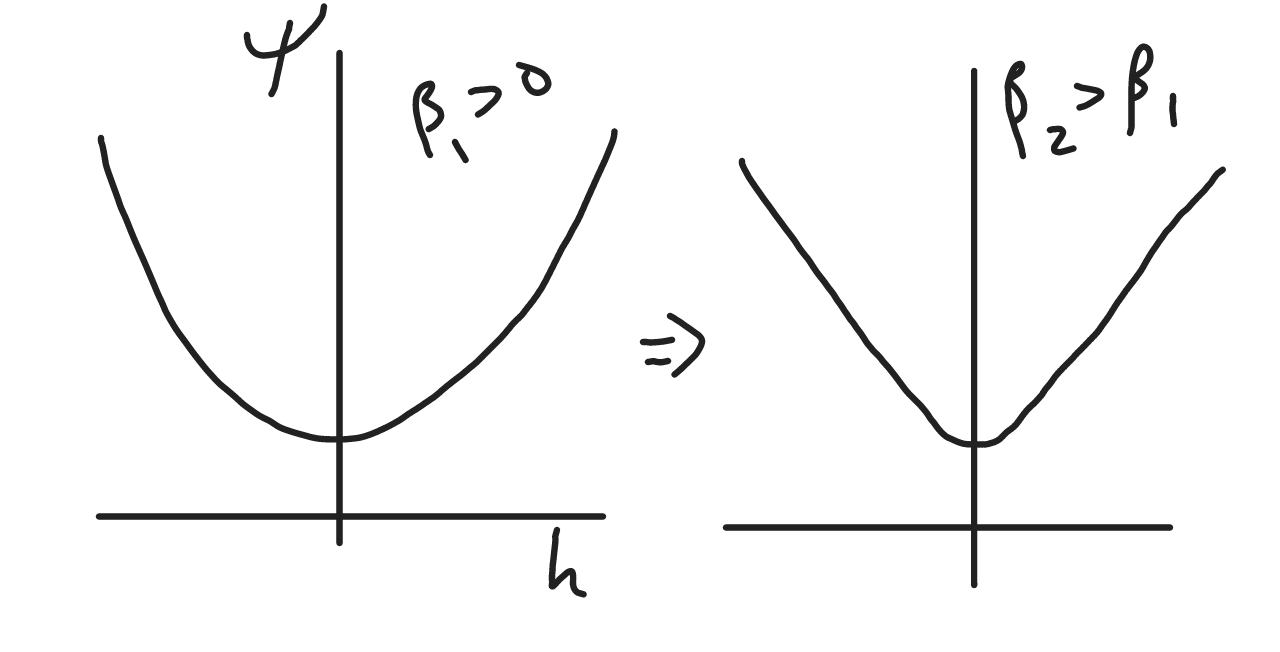
\includegraphics[scale=.25]{images/9-2}\end{center}

\begin{center}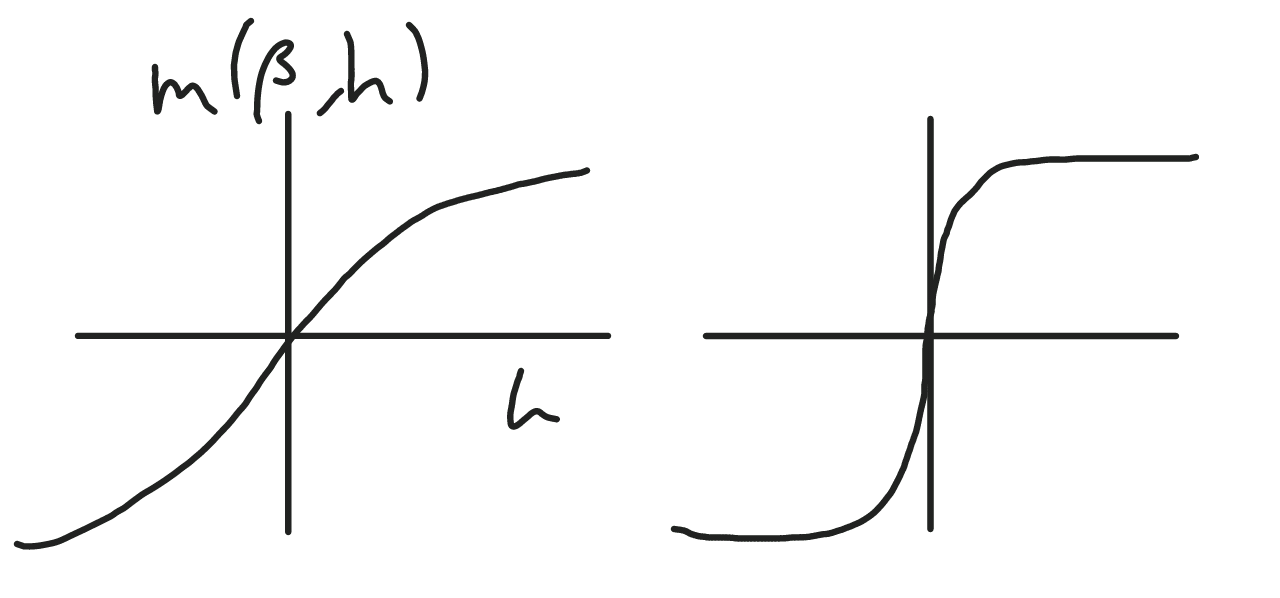
\includegraphics[scale=.25]{images/9-3}\end{center}

\begin{proof}
Take an Ising model with periodic boundary conditions $\sigma_L=\sigma_0$.
%sometimes parity matters sometimes not. Here it doesn't. 
Then (it helps to symmetrize the sum)
\begin{align*}
Z_{[0,L]}^{\text{per}} &= \sum_{\scriptsize \begin{array}{c}{\sigma_j=\pm 1}\\{\sigma_0=\sigma_L}\end{array}} e^{\beta \sum_{m=1}^L \sigma_m\sigma_{m+1} + \widehat{h} \sum_{1=1}^{L} \frac{\sigma_n+\sigma_{n+1}}{2}}\\
&=\text{tr} (A^L)
\end{align*}
where 
\be
A = 
\begin{pmatrix}
{A_{++}}&{A_{+-}}\\
{A_{-+}}&{A_{--}}
\end{pmatrix}
 = 
\begin{pmatrix}
{e^{\beta + \widehat{h}}}&{e^{-\beta}}\\
{e^{-\beta}}&{e^{\beta - \widehat{h}}}
\end{pmatrix}
.
\ee
Recall that 
\be
\text{tr}(A^L) = \sum_{\sigma_0=\sigma_L\in \pm 1} (A^L)_{\sigma_0\sigma_L} = \sum_{\scriptsize \begin{array}{c}{\sigma_i=\pm 1}\\{\sigma_0=\sigma_L}\end{array}} A_{\sigma_0,\sigma_1}A_{\sigma_1,\sigma_2}\cdots A_{\sigma_{L-1},\sigma_0}.
\ee
Since $A$ is self-adjoint, $A$ is diagonalizable. The eigenvalues have different modulus, $|\lambda_1|>|\lambda_2|$, and
\begin{align*}
\text{Tr}(A^L) &= \lambda_1^L +\lambda_2^L = \lambda_1^L\left[ {1+\left( {\frac{\lambda_2}{\lambda_1}} \right)^L} \right]\\
\frac{1}{L} \ln Z_L &= \ln \lambda_1 + \underbrace{\frac{1}{L} \ln \left[ {1+\left( {\frac{\lambda_2}{\lambda_1}} \right)^L} \right]}_{\approx \frac{1}{L}\left( {\frac{\lambda_2}{\lambda_1}} \right)^L}&\text{using }\ln (1+\varepsilon)\approx \varepsilon.\\
\lim_{L\to \infty} \frac{1}{L} \ln Z_L &=\ln \lambda_1 
%goes to 0 exp fast
\end{align*}
%if same, then identity. In modulus are not the same.
%$\la_2$ positive?

The matrix $A$ is a \index{transfer matrix}\textbf{transfer matrix} (as in a Markov chain). 
%pressure independent of boundary conditions. 
Fixing the boundary conditions $\sigma_0,\sigma_L$, we have
\be
Z_L^{b.c.} = \sum A_{\sigma_0\sigma_1}A_{\sigma_1\sigma_2}\cdots A_{\sigma_{L-1}\sigma_L} = (A^L)_{\sigma_0\sigma_L}
\ee
(Exercise: write this in terms of the eigenvalues.)
%hit on head for disagreement
\end{proof}
Consider $Z_L^{++},Z_L^{+-},Z_L^{-+},Z_L^{--}$.
Assuming the magnetic field is positive ($h>0$), the maximum is $Z_L^{++}$; if $h<0$ then the maximum is $Z_L^{--}$. We have
\be
\left| {\frac{Z^{++}-Z^{--}}{Z^{++}}} \right| \le \left| {\frac{\lambda_2}{\lambda_1}} \right|^L
\ee

%if open-ended boundary conditions, can ask the following.
With open-ended boundary conditions, the spins are an array of variables with the Markov property. If you specify a spin, then the distribution of the future does not depend on the past beyond the value of the previous spin. Thus the values form a Markov chain, and the transfer matrix is familiar from the theory of Markov chains. 

What happens beyond 1 dimension? Then the Markov property re-emerges in an interesting way. When you talk about the distribution of a finite system, it's sufficient to give the spins at the boundary. 
There is a multidimensional Markov property, specified by boundary spins. %Limiting boundary distribution,
We will arrive at the theory of Gibbs states.